\documentclass[10pt,journal]{IEEEtran}
\usepackage[letterpaper,top=1in,bottom=1in,left=.7in,right=.7in,columnsep=.2in]{geometry}
\usepackage{amsmath,amssymb,graphicx,booktabs,array,fontspec,placeins,balance}
\usepackage[hidelinks]{hyperref}
\setmainfont{Times New Roman}
\newtheorem{proposition}{Proposition}
\newtheorem{theorem}{Theorem}
\newcommand{\norm}[1]{\lVert#1\rVert}
\newcommand{\um}{\,\mu\mathrm{rad}}
\graphicspath{{results/}{../v6/results/}}
\def\MatchedRows{
R1 below & Certificate & 221 & 221 & 6 & 0 & 0.000 & 3.084 \\
R1 below & Fixed guard & 0 & 0 & 0 & 0 & 0.000 & 0.000 \\
R1 below & Parameter KF & 600 & 600 & 15 & 0 & 0.000 & 74.747 \\
R1 below & ES tracker & 600 & -- & -- & 0 & 0.000 & 42.381 \\
R1 middle & Certificate & 600 & 594 & 26 & 0 & 0.000 & 8.331 \\
R1 middle & Fixed guard & 0 & 0 & 0 & 0 & 0.000 & 0.000 \\
R1 middle & Parameter KF & 600 & 600 & 15 & 0 & 0.000 & 74.747 \\
R1 middle & ES tracker & 600 & -- & -- & 0 & 0.000 & 42.381 \\
R1 above & Certificate & 600 & 594 & 26 & 0 & 0.000 & 8.331 \\
R1 above & Fixed guard & 239 & 233 & 6 & 0 & 0.000 & 3.319 \\
R1 above & Parameter KF & 600 & 600 & 15 & 0 & 0.000 & 74.747 \\
R1 above & ES tracker & 600 & -- & -- & 0 & 0.000 & 42.381 \\
R2 below & Certificate & 0 & 0 & 0 & 0 & 0.000 & 0.000 \\
R2 below & Fixed guard & 28 & 28 & 0 & 0 & 0.000 & 0.393 \\
R2 below & Parameter KF & 600 & 600 & 22 & 0 & 0.000 & 74.748 \\
R2 below & ES tracker & 600 & -- & -- & 0 & 0.000 & 42.272 \\
R2 middle & Certificate & 0 & 0 & 0 & 0 & 0.000 & 0.000 \\
R2 middle & Fixed guard & 41 & 41 & 0 & 0 & 0.000 & 0.565 \\
R2 middle & Parameter KF & 558 & 528 & 14 & 30 & 0.000 & 68.391 \\
R2 middle & ES tracker & 558 & -- & -- & 30 & 0.000 & 38.633 \\
R2 above & Certificate & 0 & 0 & 0 & 0 & 0.000 & 0.000 \\
R2 above & Fixed guard & 0 & 0 & 0 & 0 & 0.000 & 0.000 \\
R2 above & Parameter KF & 0 & 0 & 0 & 0 & 0.000 & 0.000 \\
R2 above & ES tracker & 0 & -- & -- & 0 & 0.000 & 0.000 \\
}

\raggedbottom
\begin{document}
\title{Conditional Probe Authorization for Optical Fault Diagnosis Under Finite Actuator-Model Uncertainty}
\author{}
\maketitle
\begin{abstract}
An optical diagnostic probe can interrupt a functioning link while distinguishing pointing loss from scalar attenuation. This paper develops a conditional probe-authorization certificate for a two-axis terminal with a declared finite actuator-model set. Under fixed-offset and divergence assumptions, a bounded log-gain decline and a simultaneous sensor event, an angular-displacement enclosure yields a lower bound on sampled received power and a finite-window outage-count test. A supervisory interface refuses unsupported contracts and separates probe service from estimation, diagnosis and recovery. A development-guided admission-frontier study compares the certificate with a fixed 2-microradian guard in 7,200 trials. An additional, separately frozen 7,200-run extension evaluates parameter filtering and extremum-seeking tracking under matched time and plant conditions. In the low-noise midpoint, the certificate admits 600 probes and accepts 594 fits, while the guard admits none; 26 accepted fits miss their approximate uncertainty radius. Parameter filtering accepts 600 fits with greater angular excitation. In a reverse region the guard accepts 41 fits while the certificate refuses all. Every method has zero observed sampled outage in these restricted settings. Independent calculation replays 10,080,000 actuator steps across the two studies. The evidence supports conditional diagnostic access, not universal superiority or physical safety. Hardware calibration, continuous actuator uncertainty and robust post-probe recovery remain open.
\end{abstract}
\begin{IEEEkeywords}Optical fault diagnosis, active probing, supervisory control, finite-model uncertainty, sampled service.\end{IEEEkeywords}
\section{Introduction}
A decrease in received optical power is not a unique fault signature. Boresight displacement, reduced optical throughput and time-varying gain can produce similar scalar measurements. A controlled beam displacement can distinguish some of these causes, but it consumes link margin. On an already functioning inter-satellite link, diagnostic excitation can therefore create the service interruption it is intended to prevent. An operationally meaningful decision is whether a proposed, finite probe has a justified service budget before it is executed.

Acquisition, alignment and diagnostic identification are related but distinct problems. Acquisition searches for a previously unavailable link; extremum seeking moves toward larger measured power; active diagnosis designs excitation to distinguish parameters or hypotheses. A useful acquisition or tracking law need not deliver a calibrated fault estimate. Conversely, a well-conditioned diagnostic experiment can violate a receiver threshold. The challenge studied here is the permission between a diagnostic planner and the pointing controller, with an explicit boundary on what that permission means.

This question has established antecedents. Optical acquisition and pointing control have a substantial history \cite{guelman}. Active fault diagnosis with chance constraints allocates probabilistic constraint risk \cite{guo}. Guaranteed diagnosis of uncertain nonlinear systems can use reachable-set verification \cite{massa}, and safety-filtered extremum seeking connects optimization with barrier conditions \cite{safees}. Link-margin-aware optical scanning also optimizes acquisition choices \cite{yan}. These results rule out a broad claim that constraint-aware diagnosis or uncertainty-aware optical probing is new. They instead motivate a precise optical formulation: can a received-power lower bound authorize a finite diagnostic reference under declared actuator, optical and sensor contracts?

The proposed answer uses the power at the measured starting reference, rather than assuming that probing begins at zero pointing error. An angular-displacement enclosure bounds the change in the Gaussian beam loss. A simultaneous event covers all five sensor channels over the declared mission, so choosing the start from observed anomalies does not require treating a pointwise interval as an interval valid after selection. The actuator enclosure enumerates six discrete inertia/lag pairs and explicitly refuses possible clamp activation. The result is conditional on those contracts; it does not establish them from flight hardware.

The contributions are the following.
\begin{enumerate}
\item A reference-relative optical inequality and a sampled-outage theorem with explicit offset, divergence, gain-slope, sensor-tail and finite-model hypotheses. The centered angular bound is sharp for its stated ball geometry, while the complete power certificate can remain conservative.
\item A complete finite-model construction, candidate-selection rule and executable supervisory contract that separates authorization, fit acceptance, diagnosis and post-probe correction. Failure-closed behavior is exercised in shadow mode.
\item A reproducible admission-frontier evaluation covering both disagreement directions and controls, with an additional matched parameter-filter and extremum-seeking extension. Full state/noise records support separate numerical replay and disclosure of accepted-fit confidence misses and finite-horizon incompletion.
\end{enumerate}
These contributions are a specialized conditional formulation and evidence package, not a claim of absolute priority or universal improvement. The subsequent sections position the method, specify the model and assumptions, derive the certificate, construct the supervisor, and evaluate its operating envelope. Discussion and limitations translate the observed tradeoffs into design implications.

\section{Related Work and Research Gap}
\subsection{Optical acquisition, pointing and link margin}
Guelman \emph{et al.} address inter-satellite acquisition and pointing \cite{guelman}. Mechanical fine-pointing reviews and pointing-budget studies describe important actuator and angular-error considerations \cite{actuators,baeck}. They motivate including actuator response and sensor uncertainty; they do not calibrate the numerical terminal used here. NASA's small-spacecraft communications overview likewise supplies application context rather than evidence for this assumed unit \cite{nasa}.

Yan \emph{et al.} explicitly study link-margin-aware scanning and acquisition \cite{yan}. Recent optical work by Oh and Noh examines uncertainty-cone design with time-correlated retries \cite{oh}. Its published abstract distinguishes retry models and identifies conditions for different optimum behavior. That treatment concerns acquisition-cone/retry design; the present decision concerns a finite diagnostic reference starting from a measured power state. Only its publisher abstract and metadata were accessible for this study, so exact algorithmic overlap and faithful implementation remain unresolved. No numerical advantage over that paper is claimed.

\subsection{Constrained and guaranteed active diagnosis}
Chance-constrained diagnosis of linear stochastic systems \cite{guo} and reachability-based guaranteed diagnosis for nonlinear models \cite{massa} already connect informative input design and constraints. Their models, ambiguity objectives and guarantees differ from the scalar optical-power contract here. A fair comparison would map optical dynamics, sensing, admissible hypotheses and objectives into the original formulations. Replacing that mapping by a generic estimator and calling it a reproduction would be misleading.

Two feasible architectures are evaluated: a linear Kalman parameter filter on the transformed optical model and a washout/demodulation extremum-seeking tracker. They are explicitly adapted baselines. The former tests whether sequential parameter estimation can obtain more diagnostic access under the same trigger and time limit; the latter tests a tracking objective and carries no diagnosis acceptance credit. The added experiments do not reproduce the full chance-constrained or reachability-verified published systems.

\subsection{Supervision and uncertainty contracts}
Classical extremum-seeking stability analysis \cite{es} and modern safety-filtered extremum seeking with unknown barrier functions \cite{safees} address properties beyond a finite lookup certificate. The present supervisor is narrower: it checks whether a candidate's stated evidence supports a sampled probe-window outage count. It also exposes why a valid service permission cannot be interpreted as an accurate fault estimate or permission for a subsequent recovery maneuver.

Table~\ref{tab:prior} states verified scope and the actual reproduction status. ``Not assessed'' is not a claim that an original paper lacks physical validation. The source review remains incomplete for some recent optical work, and absolute novelty over close prior art remains unconfirmed. The research gap claimed here is consequently a concrete formulation and implementation boundary, rather than the invention of safe active diagnosis.

\begin{table*}[t]
\caption{Prior-art positioning and reproduction status. Original-paper guarantees are described at their verified level; no ranking follows from different objectives. Physical validation is not assumed from bibliographic metadata.}
\centering\footnotesize\setlength{\tabcolsep}{4pt}
\begin{tabular}{@{}p{.15\textwidth}p{.20\textwidth}p{.18\textwidth}p{.18\textwidth}p{.22\textwidth}@{}}\toprule
Method & Model / probe selection & Guarantee or objective & Physical validation assessed here & Relevant gap / reproduction status\\\midrule
Optical acquisition and pointing \cite{guelman} & Inter-satellite pointing/acquisition control & Acquisition and pointing & Not assessed in this comparison & Different decision; no faithful numerical reproduction\\
Link-margin-aware scanning \cite{yan} & Optical acquisition scan parameters & Link-margin-aware acquisition optimization & Not assessed & Diagnostic-contract mapping not reproduced\\
Correlated-retry cone design \cite{oh} & Spiral-scan acquisition and retry assumptions & Analytical optimum behavior described in abstract & Not assessed; full text unavailable & Abstract-only positioning; no numerical reproduction\\
Chance-constrained AFD \cite{guo} & Linear stochastic dynamics; informative input & Probabilistic state constraints & Not assessed & Optical nonlinear mapping absent; not reproduced\\
Guaranteed nonlinear AFD \cite{massa} & Nonlinear uncertain models; verified inputs & Reachability-based diagnosis guarantee & Not assessed & Public code exists; required tools unavailable on active path\\
Safety-filtered ES \cite{safees} & Unknown measured barrier; adaptive dither & Semiglobal safety-filtered ES analysis & Not assessed & Full barrier/filter architecture not reproduced\\
Parameter KF / conventional ES & Transformed optical parameters / washout tracking & Approximate covariance / tracking objective & Simulation only & Adapted, matched architectures evaluated; no theorem attributed to them\\
Present certificate & Gaussian optics; finite actuator members; candidate library & Conditional sampled probe service & Simulation and shadow interface only & Distinct from correct diagnosis and post-correction recovery\\\bottomrule
\end{tabular}
\label{tab:prior}
\end{table*}

\section{Terminal Model, Assumptions and Problem}
\subsection{Plant, controller and sampling convention}
The reused source terminal \cite{source} has two axes with angle $q\in\mathbb R^2$, angular rate $v$, delivered torque $a$ and PID integral $I$. Its nominal unsaturated equations are
\begin{align}
\dot q&=v,&J_a\dot v&=a-dv,\nonumber\\
\tau_a\dot a&=u_c-a,&\dot I&=q_m-r,\label{eq:plant}
\end{align}
\begin{align}
u_{\rm raw}&=-J_0k_p(q_m-r)+(d-J_0k_d)v_m-J_0k_iI,\nonumber\\
u_c&=\operatorname{clip}_{u_{\max}}(u_{\rm raw}).\label{eq:pid}
\end{align}
Clips act componentwise on torque and rate. At a rate boundary, outward acceleration is set to zero; the angle derivative uses clipped rate. Anti-windup freezes the integral derivative when the raw torque exceeds the torque limit. The model is advanced by held-disturbance RK4 with $h=0.02$~s. Each stored state is the state before that step; sensing occurs before the new reference is chosen, and the held reference and resulting torque apply to the following integration interval. Replay uses this convention, including the final next state.

The nominal controller uses $J_0$ even when the actual actuator differs. The declared actual model set is exactly
\begin{equation}
\mathcal M=\{.8,1,1.25\}\times\{1,1.5\},\quad
(J_a,\tau_a)=(J_0m_1,\tau_0m_2).
\label{eq:models}
\end{equation}
It contains six points. Membership between these points is not certified by interpolation or endpoint testing.

\subsection{Optical power and measured channels}
For boresight offset $b$, divergence $\alpha$ and positive scalar gain $g$,
\begin{align}
p&=p_0(\alpha)g\exp[-2\norm{q+b}^2/\alpha^2],\label{eq:powerplant}\\
p_0(\alpha)&=P_t\eta_o\left[1-\exp\left(-\frac{2r_a^2}{L^2\alpha^2}\right)\right].\nonumber
\end{align}
Service is available at a sampled instant when $p\geq p_{\min}$. Here $L$ is range and $r_a$ aperture radius. Receiver-side pointing, orbital propagation, atmospheric losses, queues and routing are outside this single-terminal experiment.

The measurements have separate physical noise scales:
\begin{align}
q_m&=q+\sigma_q Z_q,&[\sigma_q]&=\mathrm{rad},\nonumber\\
v_m&=v+\sigma_v Z_v,&[\sigma_v]&=\mathrm{rad/s},\label{eq:sensors}\\
p_m&=\max\{0,p(1+\sigma_p Z_p)\},&[\sigma_p]&=1.\nonumber
\end{align}
There are five scalar channels: two angles, two rates and one relative-power disturbance. The inherited kernel uses numeric noise coefficient $\sigma_q$ for the encoder and twice that numeric value for the rate. We document this source policy dimensionally as $\sigma_v=\gamma_v\sigma_q$, $\gamma_v=2~\mathrm{s}^{-1}$. This resolves the written unit mismatch without changing any inherited sensor value. It is not an independently calibrated hardware relationship. Direct source-kernel checks reproduce 2,100 sensor samples at three noise scales with zero numerical discrepancy; the new traces retain explicit rate-unit metadata.

\begin{table}[t]
\caption{Terminal values and provenance. All physical values are assumptions; source-derived values describe implementation rather than independent calibration.}
\centering\footnotesize\setlength{\tabcolsep}{4pt}
\begin{tabular}{@{}p{.36\columnwidth}p{.40\columnwidth}p{.17\columnwidth}@{}}\toprule
Quantity & Value & Provenance\\\midrule
Range / aperture diameter & 800 km / 0.10 m & Assumed\\
$P_t,\eta_o,\alpha$ & 0.5 W, 0.4, $20\um$ & Assumed\\
$\alpha$ interval & $[18,22]\um$ & Assumed\\
Aligned $p_0$, $p_{\min}$ & 3.9062, 1.5 $\mu$W & Derived / assumed\\
$J_0,d,\tau_0$ & .002 kg m$^2$, .004 N m s/rad, .08 s & Assumed\\
$k_p,k_d,k_i$ & 64 s$^{-2}$, 14 s$^{-1}$, 8 s$^{-3}$ & Source-derived\\
Torque / rate limit & $2~\mu$N m / $120\um$/s & Assumed\\
Base $\sigma_q,\sigma_v$ & $.08\um$, $.16\um$/s & Source policy\\
Base $\sigma_p$, coupling $\gamma_v$ & .008, 2 s$^{-1}$ & Source policy\\
Sample / mission & .02 s / 14 s ($N=700$) & Protocol\\
Prior $\norm b$, maximum gain & $30\um$, 1.05 & Assumed\\
Working / acquisition budget & 0 s / 4 s & Protocol\\\bottomrule
\end{tabular}
\label{tab:model}
\end{table}

\subsection{Numbered assumption contract}
The theorem below uses the following hypotheses.
\begin{enumerate}
\item[A1.] The starting power is positive; $b$ and $\alpha$ remain constant during the candidate window; $\alpha\in[\alpha_-,\alpha_+]$ and $\norm b\leq b_{\max}$.
\item[A2.] $0<g(t_0)\leq g_{\max}$ and $\log[g(t_0+s)/g(t_0)]\geq-\ell s$ at all evaluated samples, for declared $\ell\geq0$.
\item[A3.] Actual $(J_a,\tau_a)$ belongs to \eqref{eq:models}; the source sampled dynamics and nominal controller apply. The initial state is zero, pre-probe reference is zero, and there is at most one attempt per mission.
\item[A4.] Encoder and rate bias are zero. All five standardized sensor disturbances have the declared marginal Gaussian tails and correct scales over all $N$ mission samples. Cross-channel or temporal independence is not needed for the union bound.
\item[A5.] Candidate RK4-stage torque and rate enclosures lie strictly within their clamps. Candidate duration fits the declared horizon. Optical and sensor evidence is valid for the requested window.
\end{enumerate}
A simulation record can check injected histories against this contract, but cannot establish the physical truth of A1--A5 for a real terminal. Evidence references are required by the supervisory interface; mere reference presence does not authenticate calibration or future fault constancy.

\begin{table}[t]
\caption{Recurring notation and dimensions.}
\centering\footnotesize
\begin{tabular}{@{}p{.25\columnwidth}p{.68\columnwidth}@{}}\toprule
Symbol & Meaning / dimension\\\midrule
$h,N,\delta$ & Sample time (s), mission samples, failure allowance\\
$e_0,d_i$ & Starting angular error, delivered increment (rad)\\
$c,R,\bar d_i,r_i$ & Centers and radii of error/increment balls (rad)\\
$\overline D_i$ & Upper change in squared angular loss (rad$^2$)\\
$\ell,\kappa,\eta$ & Log-gain decline (s$^{-1}$), tail quantile, relative envelope\\
$\underline p_i,B$ & Power lower bound (W), sampled outage budget (s)\\
$M,H,K$ & Number of models, window samples, candidates\\
$\rho_x,F,C_b$ & State box radii, projected information, offset covariance\\\bottomrule
\end{tabular}
\end{table}

\subsection{Authorization objective and four separate properties}
Given a candidate reference, measured start and its proposed displacement enclosure, compute $\underline p_i$ such that actual sampled window outage obeys
\begin{equation}
h\sum_{i=0}^{H-1}\mathbf1\{p_i<p_{\min}\}
\leq h\sum_{i=0}^{H-1}\mathbf1\{\underline p_i<p_{\min}\}\leq B
\label{eq:objective}
\end{equation}
under the contract. This authorizes sampled service for that probe only. It does not bound the offset estimation error, guarantee a correct diagnosis, or authorize a post-probe correction. The estimator and recovery logic in Fig.~\ref{fig:flow} remain separate from the blue permission path.

\begin{figure*}[t]
\centering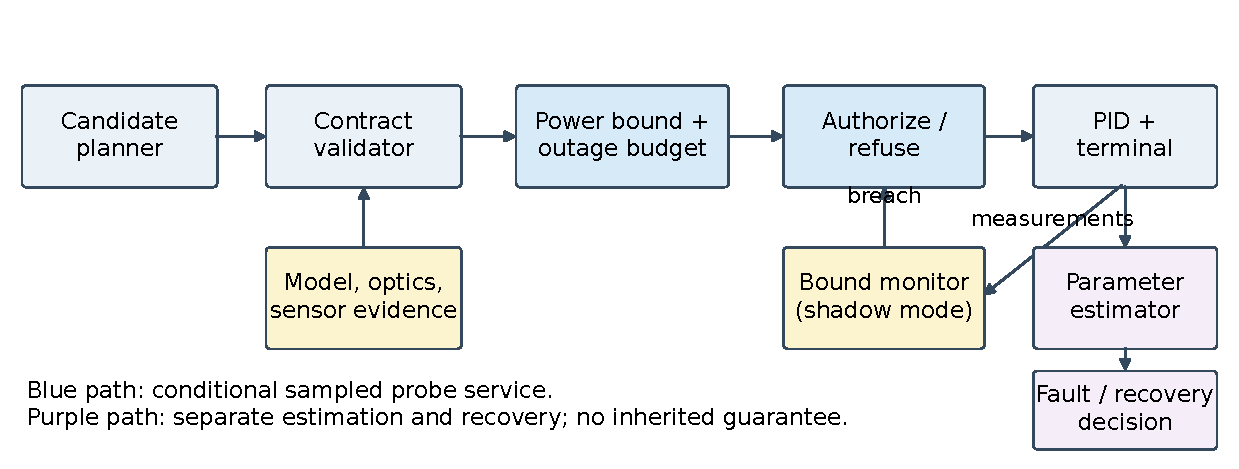
\includegraphics[width=\textwidth]{information_flow.pdf}
\caption{Information flow and guarantee boundary. Evidence validation precedes conditional permission. Estimation and recovery consume measurements but do not inherit the probe-window service theorem. The supplied implementation is a simulation/shadow interface.}
\label{fig:flow}
\end{figure*}

\section{Conditional Optical Service Certificate}
\subsection{Reference-relative identity and angular geometry}
Let $e_0=q(t_0)+b$ and $d_i=q(t_0+s_i)-q(t_0)$. For fixed $b,\alpha$ and positive starting power, the exact identity is
\begin{equation}
\log\frac{p(t_0+s_i)}{p(t_0)}=
\log\frac{g(t_0+s_i)}{g(t_0)}-
\frac{2}{\alpha^2}\left(2e_0^Td_i+\norm{d_i}^2\right).
\label{eq:identity}
\end{equation}
The cross term retains the true starting angular error. Omitting it, or replacing delivered motion by commanded motion without an enclosure, can overstate the available margin.

\begin{proposition}[Angular loss over two balls]
Suppose $e_0\in\mathcal B(c,R)$ and $d_i\in\mathcal B(\bar d_i,r_i)$ with nonnegative Euclidean radii. Then $2e_0^Td_i+\norm{d_i}^2\leq\overline D_i$, where
\begin{align}
\overline D_i={}&2c^T\bar d_i+2R\norm{\bar d_i}+\norm{\bar d_i}^2\nonumber\\
&+2(\norm{c+\bar d_i}+R)r_i+r_i^2.
\label{eq:Dgeneral}
\end{align}
For $c=0$, the exact maximum is
\begin{equation}
D_{\max,i}=2R(\norm{\bar d_i}+r_i)+(\norm{\bar d_i}+r_i)^2.
\label{eq:Dcenter}
\end{equation}
\end{proposition}
\emph{Proof:} Write $e_0=c+u$, $d_i=\bar d_i+w$, $A=\norm{\bar d_i}$, $C=\norm{c+\bar d_i}$. Exact expansion gives
\begin{align}
\overline D_i-(2e_0^Td_i+\norm{d_i}^2)
={}&2(RA-u^T\bar d_i)\nonumber\\
&+2(r_iC-(c+\bar d_i)^Tw)\nonumber\\
&+2(Rr_i-u^Tw)+(r_i^2-\norm w^2).
\end{align}
Each summand is nonnegative by Cauchy--Schwarz, $\norm u\leq R$ and $\norm w\leq r_i$. For $c=0$, $A>0$, the choice $u=R\bar d_i/A$, $w=r_i\bar d_i/A$ attains \eqref{eq:Dcenter}. If $A=0$, use $u=Rz$, $w=r_i z$ for any unit vector $z$. These constructions include either radius zero and the singleton cases. Noncentered sharpness is not asserted.\hfill$\square$

All terms in $\overline D_i$ have dimension rad$^2$. Combining \eqref{eq:identity} with A1--A2 and $p(t_0)\geq\underline p_0$ gives
\begin{equation}
\underline p_i=\underline p_0\exp\left[-\ell s_i-
\frac{2\max(\overline D_i,0)}{\alpha_-^2}\right].
\label{eq:lower}
\end{equation}
For nonnegative angular loss, the smallest allowed divergence is conservative. If its upper bound is negative, replacing it by zero discards guaranteed improvement and avoids reversing the divergence inequality. Sharpness of the centered angular geometry does not imply tightness of \eqref{eq:lower}: optical priors, initial-power intervals and actuator uncertainty can be mutually coupled and conservatively separated.

\subsection{Simultaneous sensor event and numeric calibration}
Define the mission event
\begin{equation}
\mathcal E=\{ |Z_{k,j}|\leq\kappa\quad\text{for all }0\leq k<N,\ 1\leq j\leq5\}.
\end{equation}
With standard Gaussian marginal tails,
\begin{align}
\kappa&=\Phi^{-1}\!\left(1-\frac{\delta}{10N}\right),\nonumber\\
\Pr(\mathcal E^c)&\leq\sum_{k,j}\Pr(|Z_{k,j}|>\kappa)\leq\delta.
\label{eq:event}
\end{align}
The exact implementation uses $\sqrt2\operatorname{erfc}^{-1}[\delta/(5N)]$. Here $\delta=0.01$, $N=700$ for samples $0,.02,\ldots,13.98$~s, and $\kappa=4.680831082738$ (rounded). Each two-sided scalar tail is $\delta/(5N)=2.857142857\times10^{-6}$. This is a mission event, not a separate 99\% interval at each measurement. No independence assumption enters the union bound.

For $\eta=\kappa\sigma_p<1$, on $\mathcal E$,
\begin{equation}
\underline p_0=\frac{p_m(t_0)}{1+\eta}\leq p(t_0)\leq
\frac{p_m(t_0)}{1-\eta}=\overline p_0.
\label{eq:interval}
\end{equation}
The interval holds simultaneously at every index, hence also at an observation-selected trigger $\tau$. In particular,
\begin{equation}
\{\overline p_\tau<p_{\min}\leq p_\tau\}\subseteq\mathcal E^c.
\label{eq:falseenable}
\end{equation}
This avoids optional-selection misuse of a pointwise interval; it does not imply an exact coverage probability conditional on having triggered or accepted a fit.

An acquisition budget is enabled only when $\overline p_0<p_{\min}$. A straddling interval keeps the working-link budget. On $\mathcal E$ with positive power and $\eta<1$, the multiplier in \eqref{eq:sensors} is positive, so zero clipping is inactive. At true zero power, $p_m=0$ and the detector-floor rule refuses a probe. If $\eta\geq1$, the upper endpoint is unbounded and cannot enable acquisition.

\subsection{Starting-error enclosure and service theorem}
The source selector uses a centered enclosure. On $\mathcal E$, $\epsilon_q=\sqrt2\kappa\sigma_q$ bounds the encoder-vector error. Combining the offset prior with the measured angle gives $R_{\rm prior}=b_{\max}+\norm{q_m(t_0)}+\epsilon_q$. The optical identity at the start gives a second valid radius,
\begin{equation}
R_{\rm power}=\alpha_+\sqrt{\frac12\max\!\left\{0,\log\frac{p_{0,+}g_{\max}}{\underline p_0}\right\}},
\end{equation}
where $p_{0,+}$ is the maximum aligned power over the declared divergence interval. Thus $R=\min(R_{\rm prior},R_{\rm power})$ is valid whenever both priors are consistent. The positive-part operator is the implementation's conservative nonnegative convention; a physically inconsistent empty prior must not be treated as a new calibrated state estimate.

\begin{theorem}[Conditional sampled probe service]
Consider a candidate starting at a possibly observation-selected sample $\tau$ and ending within the $N$-sample mission. Suppose A1--A5 hold, the starting-error ball is valid, and for each window sample the delivered increment is contained in $\mathcal B(\bar d_i,r_i)$. On $\mathcal E$, let $\underline p_i$ be \eqref{eq:lower} using \eqref{eq:interval} and Proposition~1. Then $p_{\tau+i}\geq\underline p_i$. If the selector admits only candidates satisfying
\begin{equation}
\widehat O=h\sum_{i=0}^{H-1}\mathbf1\{\underline p_i<p_{\min}\}\leq B,
\end{equation}
the actual sampled probe-window outage is at most $B$. For otherwise valid contracts, any failure of this implication due to the stipulated sensor event is contained in $\mathcal E^c$, with unconditional mission probability at most $\delta$.
\end{theorem}
\emph{Proof:} On $\mathcal E$, the starting-power and error enclosures hold at every possible start. Proposition~1 bounds the angular-loss term at each candidate sample. A1--A2 then turn \eqref{eq:identity} into \eqref{eq:lower}. Pointwise, $\mathbf1\{p_{\tau+i}<p_{\min}\}\leq\mathbf1\{\underline p_i<p_{\min}\}$. Multiplying by $h$ and summing proves the outage implication. Simultaneity permits the selected start, and \eqref{eq:event} bounds its event-complement probability.\hfill$\square$

\emph{What the theorem does not prove:} It is not a continuous-time intersample guarantee, a formally rounded floating-point enclosure, a probability conditional on estimator acceptance, or a certificate of correct diagnosis. It establishes neither actual hardware calibration nor recovery after a later correction. Wrong tails, bias, continuous actuator parameters outside the finite set, or an offset changing within the window invalidate its premises. Figure~\ref{fig:geometry} illustrates the actual recorded quantities, not a new experiment.

\begin{figure*}[t]
\centering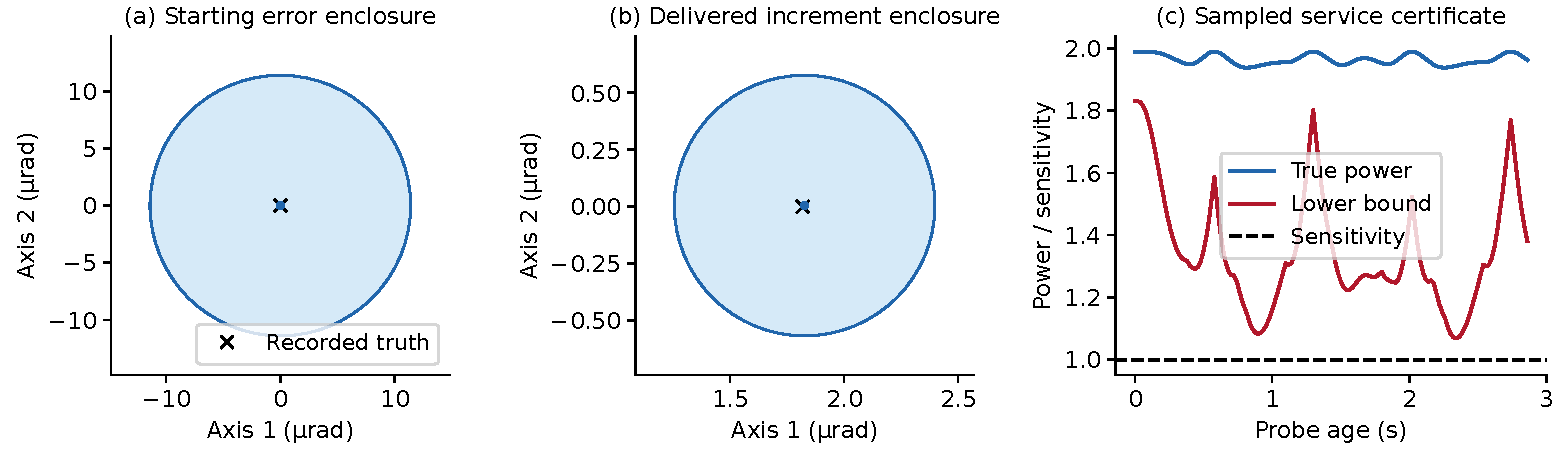
\includegraphics[width=\textwidth]{certificate_geometry.pdf}
\caption{Certificate geometry and actual power for region~1 midpoint, seed~7001, nominal actual actuator. The initial-error ball and one delivered-increment ball are in different coordinate planes; crosses show recorded truth. Panel (b) uses the middle probe sample. Panel (c) shows true and bounded power over the same recorded probe. Centers/radii are exported in the supplementary figure-source record.}
\label{fig:geometry}
\end{figure*}

\section{Finite-Model Enclosure and Authorization Algorithm}
\subsection{Sampled actuator maps}
For one unsaturated axis, let $x=(q,v,a,I)^T$ and $w=(r,n_q,n_v)^T$. With $J_a=J_0m_1$, $\tau_a=\tau_0m_2$,
\begin{equation}
A_m=\begin{bmatrix}
0&1&0&0\\0&-d/J_a&1/J_a&0\\
-J_0k_p/\tau_a&(d-J_0k_d)/\tau_a&-1/\tau_a&-J_0k_i/\tau_a\\
1&0&0&0
\end{bmatrix},
\end{equation}
\begin{equation}
B_m=\begin{bmatrix}0&0&0\\0&0&0\\J_0k_p/\tau_a&-J_0k_p/\tau_a&(d-J_0k_d)/\tau_a\\-1&1&0\end{bmatrix}.
\end{equation}
The angle and rate disturbance columns carry different input units. Form $\mathcal A_m=\begin{bmatrix}A_m&B_m\\0&0\end{bmatrix}$ and
\begin{equation}
P_4(h\mathcal A_m)=I+h\mathcal A_m+
\frac{h^2\mathcal A_m^2}{2}+\frac{h^3\mathcal A_m^3}{6}+\frac{h^4\mathcal A_m^4}{24}.
\end{equation}
Its upper blocks are the exact map $A_{d,m},B_{d,m}$ of this held-input RK4 implementation, rather than the exact continuous-time exponential. Write $B_{dn,m}$ for its sensor columns and $n_{\max}=\kappa(\sigma_q,\sigma_v)^T$.

Starting from zero state, a coordinatewise finite-impulse bound is
\begin{equation}
\rho_{x,m}=\sum_{j=0}^{N-1}|A_{d,m}^{j}B_{dn,m}|n_{\max}.
\label{eq:impulse}
\end{equation}
The nonnegative mission-length sum overbounds all shorter pre-trigger histories. Mean trajectories are propagated for each model with the proposed reference; the nominal mean is $\mu_{0,i}$ and each member's mean is $\mu_{m,i}$. A two-axis angular radius around the nominal mean is
\begin{equation}
\rho_{q,i}=\max_{m\in\mathcal M}\left[
\norm{\mu_{m,i}^{q}-\mu_{0,i}^{q}}+\sqrt2\rho_{x,m}^{q}\right].
\end{equation}
The delivered increment uses $\bar d_i=\mu_{0,i}^{q}-q_m(t_0)$ and $r_i=\rho_{q,i}+\epsilon_q$. Triangle containment then includes the measured-start error. This construction depends on the zero initial state and zero pre-probe reference; it is not a restart formula for an arbitrary prior maneuver.

\subsection{Why stage constraints are necessary}
The linear map applies only while the plant's nonlinear clips and anti-windup are inactive. For each RK4 stage, derive its state as $S_lx+T_lw$, with $S_1=I,T_1=0$ and, successively,
\begin{equation}
S_l=I+\beta_l A_m S_{l-1},\quad
T_l=\beta_l(A_mT_{l-1}+B_m),
\end{equation}
where $\beta_2=\beta_3=h/2$, $\beta_4=h$. The raw-torque row is $C_u=(-J_0k_p,d-J_0k_d,0,-J_0k_i)$ plus the direct reference and sensor terms. Finite-impulse sums of $C_uS_lA_{d,m}^jB_{dn,m}$ bound its history-driven uncertainty; direct stage-input terms are added. The rate row is handled identically. Every axis, stage, sample and finite member must satisfy strict torque/rate containment.

Induction establishes consistency: if all previous sampled states belong to the enclosure and each proposed stage remains inside its clamps, the clipped plant follows the unsaturated RK4 stage equations and the next state belongs to the propagated enclosure. If a stage cannot be enclosed strictly, the candidate is refused; the library does not claim to enclose an arbitrary saturated trajectory. Independent calculations reproduce six maps, eight previously audited candidates/tubes and 33,024 stage checks. Full stage algebra and numerical differences are in the supplement.

\subsection{Candidate selection and estimation}
The present library contains four amplitudes $\{2,4,6,8\}\um$, one dwell length .36~s and eight balanced dwells per candidate. Constraint and approximate information checks precede the service calculation. The latter requires an estimated offset radius no greater than $1\um$; it is a design heuristic, not an estimator-coverage theorem. Among admissible candidates, the source cost is duration plus $0.03h\sum_i\norm{\mu_{0,i}^{q}/(1\um)}^2$, with the numerical cost coefficient interpreted in the source's chosen seconds units. This is a heuristic ranking, not electrical energy minimization.

For the diagnostic fit, let $Q_i=q_{m,i}^T/\alpha$ and remove affine temporal nuisance using an orthogonal projection $P$. With exact regressors, $F=Q^TPQ\succ0$ determines identifiability. For independent Gaussian log noise of variance $\sigma^2$ and exact regressors, the offset covariance is $C_b=\alpha^2\sigma^2F^{-1}/16$; a 95\% enclosing radius is $\sqrt{5.991464547\lambda_{\max}(C_b)}$. The implemented iterated feasible GLS instead uses noisy angle regressors and approximate transformed multiplicative-noise variance. Residual, radius, offset-prior and gain-range checks determine fit acceptance. Consequently its radius remains approximate even when the service certificate is valid.

\subsection{Contract interface and pseudocode}
The evidence interface records finite-model membership, angle/rate/power units, marginal-tail/scales, mission start/horizon, validity expiry and references for actuator, sensor, optical and window contracts. The new wrapper additionally refuses a window that would extend beyond the remaining mission horizon. These checks verify metadata consistency; validating the referenced reports belongs to an external evidence authority. Synthetic simulation references are refused for physical deployment.

\begin{table}[t]
\caption{Supervisor algorithm. All permissions remain conditional on evidence truth. ``Fallback'' means a separately validated neutral-controller policy.}
\centering\footnotesize
\begin{tabular}{@{}p{.94\columnwidth}@{}}\toprule
\textbf{Inputs:} measurements/history, candidate library, finite-model maps, evidence contracts, mission time, $p_{\min}$, budgets.\\\midrule
1. Check evidence presence, authority/provenance, expiry, units, model membership and remaining horizon. Refuse on failure.\\
2. Form the simultaneous power interval. Refuse detector-floor/invalid intervals. Enable acquisition budget only if its upper endpoint is below $p_{\min}$.\\
3. For each candidate: reject invalid RK4-stage clamps, failed information checks or unavailable enclosure. Form initial-error ball, increment balls and $\underline p_i$.\\
4. Reject candidates with $h\sum_i\mathbf1\{\underline p_i<p_{\min}\}>B$. If none remain, abstain. Otherwise choose minimum source cost and issue conditional probe permission only.\\
5. During the probe, compare measured power's upper envelope with the predicted true-power lower bound. On breach: mark uncertified, inhibit repeated probing, request validated fallback.\\
6. After completion, estimate and report fit acceptance/uncertainty separately. Do not infer verified diagnosis or recovery authorization from step~4.\\\bottomrule
\end{tabular}
\label{tab:algorithm}
\end{table}

A monitor breach means $p_m/(1-\eta)<\underline p_i$, up to numerical tolerance. It signals inconsistency, not guaranteed immediate restoration of service. The current plant experiments evaluate selection and recorded outcomes; the monitor is replayed in shadow mode and does not constitute a closed-loop physical protection test.

\subsection{Computational scaling}
For fixed state dimension, precomputing history impulse/stage sums costs $O(MN)$ and propagating $K$ candidate mean/stage trajectories costs $O(KMH)$. Source loops recompute some impulse sums per candidate, giving $O(KM(N+H))$ for the current implementation. At a trigger, candidate lower-bound evaluation costs $O(KH)$; per-sample monitoring is $O(1)$. Storing all candidate means/radii costs $O(KH)$, apart from optional full raw traces. Reported desktop timings exclude offline library construction and are descriptive, not embedded worst-case timing or a flight-computing qualification.

\section{Experimental Protocol}
\subsection{Development map and confirmation selection}
The study's primary estimand is the difference in diagnostic admission at development-selected boundaries, not global recovery performance. A deterministic map evaluates seven standard-deviation scales $\{.25,.5,.75,1,1.25,1.5,2\}$, four log-gain decline bounds $\{0,.045,.09,.15\}$~s$^{-1}$ and 241 measured power/sensitivity ratios from 1 to 2.2 in increments .005. All 6,748 points are retained. The map uses a measured zero angle to isolate admission geometry and is not a causal plant simulation.

Before the original confirmation outcomes, the protocol chooses the lexicographically first noise/bound group with each disagreement direction, the midpoint of its band and adjacent below/above controls. This representative-band choice is a disclosed narrowing from an initial proposal to confirm every transition. Both directions and all controls are retained. Region~1 has noise scale .25, $\ell=0$, and power ratios 1.905, 1.990, 2.075. Region~2 has scale .75, $\ell=0$, and ratios 2.175, 2.1875, 2.200. Thus $\sigma_q$ is .02 or $.06\um$, $\sigma_v$ is .04 or $.12\um$/s, and $\sigma_p$ is .002 or .006. Low noise and nondeclining gain are stronger assumptions than in the preserved drift benchmark.

The map's measured ratio is translated into a post-change physical gain $g=({\rm ratio})p_{\min}/p_0$. Gain is initially one and changes at $t=2$~s to that constant level. Actual boresight offset is zero. The link is usable in these tests, so subsequent evidence acquisition earns no recovery credit. State is initialized at zero. The causal trigger requires three consecutive samples with absolute log residual exceeding .18, after $t>1$~s; the residual uses measured angle/power and nominal optics. Decisions have no true fault label, true offset or actual mismatch as input.

\subsection{Methods and matched resource conditions}
The original confirmation compares the uncertainty-aware diagnostic selector (UAD, labeled ``Certificate'') with a fixed-$2\um$ guard. The guard retains the same starting-power interval, centered optical bound, information check, cost and offline constraint checks, but substitutes $2\um+\epsilon_q$ for the delivered-motion radius. It is an explicitly heuristic margin, not a proven enclosure. Both select balanced eight-dwell candidates with a 2.88-s excitation limit.

An additional protocol is frozen after the original selector outcomes are known, but before any new baseline outcome. It evaluates parameter KF and conventional extremum seeking at the identical six settings, seeds, six actual models, Gaussian disturbances, trigger and 2.88-s time limit. This extension is exploratory; the four methods were not jointly predeclared before the original confirmation. Source hashes and both protocols preserve the sequence.

The parameter filter uses a four-state transformed model: two offset coefficients, a current nuisance intercept and a log-gain slope. Sequential linear updates use first-order angle/power variance, Joseph covariance updates and process tuning zero. Its fixed diagnostic waveform has $6\um$ amplitude and eight .36-s dwells. It has no service certificate. The ES tracker uses $4\um$ sinusoidal dither at .25/.4~Hz, unit-rate washout, demodulation, .7-rate gradient filtering and adaptation gain .3. It reports tracking/correction outcomes, not a diagnostic fit. These tunings are inherited from disjoint development seeds 41--45 and were not retuned on extension outcomes. The short window is less than a full period of its slow sinusoid; native-duration tracking behavior is therefore considered separately in the supplement.

All methods use the common nominal PID, physical torque/rate/command constraints and measured information boundary. Equal time does not imply equal realized angular energy or equal diagnostic objectives. The filter's larger waveform and absence of service refusal are explicit differences; observed success does not certify an unsafe trajectory, nor does a missing certificate itself demonstrate failure. The original source's finite-horizon behavior is retained: a probe triggered too late can be incomplete at 14~s. Such records have no completed fit and are counted separately rather than forced into rejection.

\subsection{Seeds, endpoints and paired statistics}
For each setting and method, seeds 7001--7100 are paired across all six actual actuator pairs. Each two-method study contains $6\times100\times6\times2=7,200$ runs; together they contain 14,400, with 600 records per setting/method. Reusing common random numbers couples the comparisons without treating six fixed model outputs as independent random subjects.

The protocol records selection/authorization, completed-fit acceptance, approximate-confidence misses, sampled mission and probe-induced outage, angular excitation $h\sum_{k\in\mathrm{probe}}\norm{q_k}^2$, and certificate slack. Angular excitation is reported in $\mu$rad$^2$~s and is not electrical energy. Slack is the per-trace median $(p-\underline p)/p_{\min}$, summarized across selected traces. Incompletion is an additional finite-horizon accounting endpoint exposed by the new replay audit; historical per-run values are unchanged.

Paired differences average the six fixed-model contrasts within each seed, then resample the 100 seed units 5,000 times. Percentile 95\% intervals and approximate Bonferroni percentile limits over six settings are supplied. Adjustment is separately scoped per comparator and outcome; it does not cover every endpoint jointly and is not an exact small-sample confidence guarantee. ES receives no fit-acceptance comparison because it has no estimator output. The complete rows and intervals are supplied rather than selecting only favorable comparisons.

\subsection{Evidence categories and independent calculation}
Each new trace retains pre-step eight-state history, next held reference, final state, all standardized disturbances, true offset/gain, actual and measured power/angle, commanded torque, candidate bound and fit. New baseline traces additionally label the rate units explicitly. Separate NumPy code reconstructs optical power, trigger timing, metrics and each RK4 step including stage saturation and anti-windup. This checks the same sampled model independently; it does not physically replicate it.

A calculated UAD bound is ``within-premise'' when all required histories exist and numeric premise checks pass under the declared simulator. A known failed premise gives ``out-of-model'' precedence; otherwise missing required histories give ``unverified.'' Noncertificate baselines are not relabeled certified just because no outage occurs. Distributional calibration and model truth remain assumptions even for a within-premise record. Sensitivity evidence, earlier incomplete histories and corrected historical statistical exports belong to a separate evidence category documented in the supplement, rather than enlarging the confirmation denominator.

\begin{figure*}[t]
\centering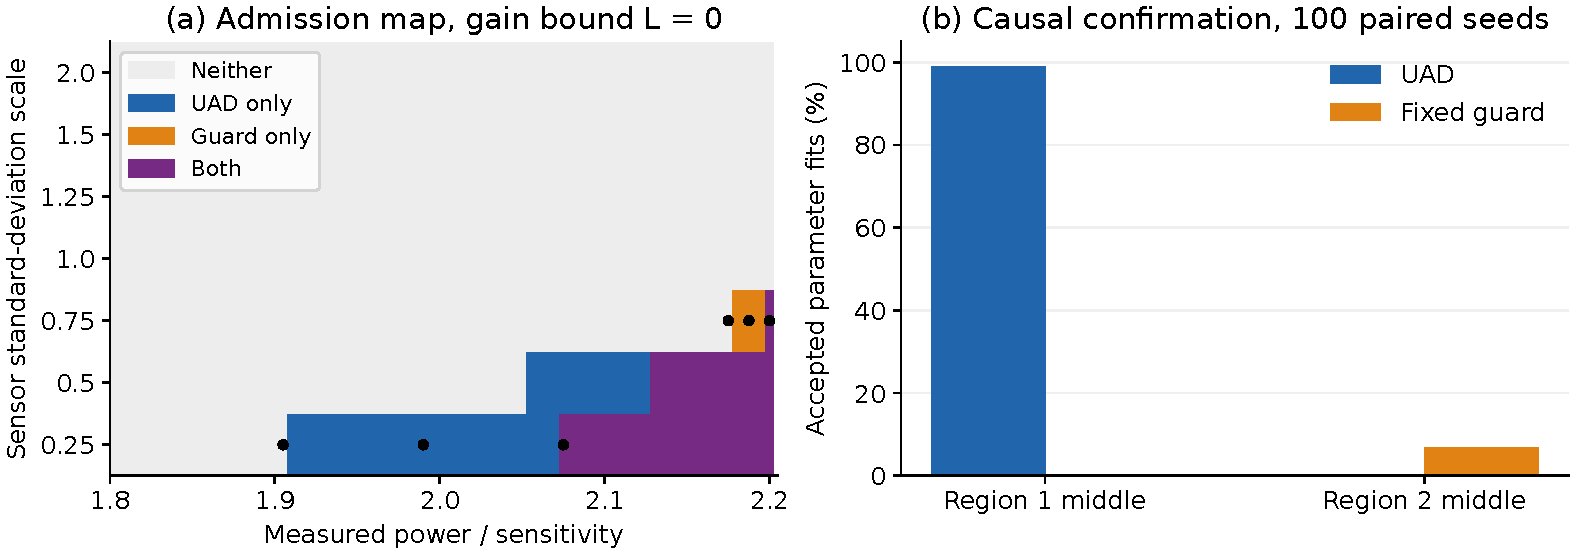
\includegraphics[width=.96\textwidth]{admission_confirmation.pdf}
\caption{Preserved development-map zoom and original two-selector midpoint confirmation. All six chosen settings are marked, including the controls; the full 6,748-point map is supplementary. The right panel concerns accepted fits only. The additional filter/ES extension is shown separately in Fig.~\ref{fig:matched}.}
\label{fig:frontier}
\end{figure*}

\section{Results}
\subsection{Do the admission rules disagree?}
Figure~\ref{fig:frontier} establishes both directions in the deterministic map. The certificate's model-derived radius can be smaller than the fixed margin in one regime and more restrictive in another. It is not uniformly a looser or stricter version of the guard. The causal experiment further changes the distribution of starting measurements: a three-sample residual trigger selects measurements from the anomaly tail. Consequently deterministic band membership does not guarantee that every causal trajectory reaches the mapped admission state.

\subsection{Paired causal confirmation and controls}
Table~\ref{tab:matched} gives all six settings for all four methods, preserving the original two-selector counts and separating the later extension. At region~1's midpoint, the certificate selects 600/600 probes and accepts 594/600 fits, whereas the guard selects none. The paired acceptance-fraction difference is .990; the original descriptive 95\% interval is $[.970,1.000]$, with approximate six-setting adjusted limits $[.960,1.000]$. This is additional diagnostic access under the specified assumptions, not faster recovery of a failed link.

The controls show how selected states affect admission: the certificate selects 221 below the first band midpoint and 600 above it; the guard selects zero below and 239 above. At the reverse midpoint, the certificate refuses every probe while the guard selects and accepts 41/600. The reverse below control gives 28 guard acceptances; above, neither method triggers or selects. No guard-only admission in this study exhibits sampled outage, so it cannot be described as demonstrated unsafe. Every row has zero actual sampled outage and zero measured probe-induced sampled outage. This selected simulated population does not provide a physical reliability rate.

\begin{table*}[t]
\caption{All matched settings, each with 100 seeds and six fixed actual models ($n=600$ per row). S: selected probes; A: accepted completed fits; C: accepted offsets outside approximate radius; I: incomplete probes at 14~s. ES has no fit output (dashes). O is mean actual sampled outage after 2~s; E is mean angular excitation. The filter/ES rows are a later, separately frozen extension, not jointly predeclared confirmation.}
\centering\small\setlength{\tabcolsep}{10pt}
\begin{tabular}{llrrrrrr}\toprule
Setting & Method & S & A & C & I & O (s) & E ($\mu$rad$^2$ s)\\\midrule
\MatchedRows
\bottomrule\end{tabular}
\label{tab:matched}
\end{table*}

\subsection{Certificate scope and numerical replay}
Across the original confirmation, 1,421 UAD probes have calculated bounds and complete within-premise histories, with zero observed bound violations. There are no out-of-model or unverified UAD bound records in this particular dataset. The 7,200 new baseline records are noncertificate or no-probe records; they do not enlarge that count. Shadow replay exercises 204,624 monitor samples from those UAD probes without an observed breach. This is a check of supplied simulation evidence, not a closed-loop fallback demonstration.

The original separate replay covers 5,040,000 actuator steps with maximum absolute state-coordinate discrepancy $3.39\times10^{-21}$. The new extension independently replays another 5,040,000 steps with maximum discrepancy $1.36\times10^{-20}$. Across the two studies this is 10,080,000 checked steps. The unit audit also agrees exactly on 2,100 direct kernel sensor samples. These numerical agreements support consistency between source, saved trajectories and the independent calculation. They are neither a floating-point rounding proof nor evidence of a calibrated physical terminal.

\subsection{Estimator reliability and confidence misses}
At the first midpoint, 26 of 594 accepted UAD offsets lie outside the reported approximate radius (4.38\% of accepted fits). Six completed fits are rejected. The median accepted absolute gain error is $2.50\times10^{-4}$, but good gain estimates do not prove every offset or fault label correct. Conditional coverage after fitting and acceptance is not the exact-regressor calculation used to motivate the radius.

The difference has identifiable modeling reasons: regressors contain encoder noise; the log of multiplicative power noise is only approximately Gaussian; angle-noise variance and mean corrections are truncated approximations; feasible GLS uses estimated weights; and residual/radius selection changes the population of accepted records. This list explains why exact 95\% coverage cannot be transferred. It is not an attribution of each observed miss to one isolated cause; such causal attribution would require additional controlled ablations. The observed rate does not itself demonstrate calibration. In particular, the service theorem does not condition on the estimated covariance and cannot repair estimator bias.

The median trace-median UAD power slack at the same midpoint is $0.657657p_{\min}$. This substantial conservatism reflects separate worst cases in initial error, divergence, gain decline, finite-model motion and sensor event. The bound serves as a permission test rather than an accurate predictor of instantaneous received power.

\subsection{Premise violations and sensitivities}
A separate preserved 50-seed affine-drift sensitivity dataset is summarized consistently in Fig.~\ref{fig:sensitivity}; it is not pooled with the admission-frontier study. With nominal sensing UAD accepts 46/50 fits and one misses its approximate radius. Injecting unmodeled angle bias $[2,-1]\um$ gives 39 accepted fits; all 39 miss the radius and exceed $1\um$ actual error. Scaling the declared noise levels by five leads to no accepted UAD fits. The latter is abstention in this dataset, not proof that any unmodeled disturbance will be detected.

Bias also has a structural explanation. If $q_m=q+\beta$, then $q+b=q_m+(b-\beta)$; scalar optical power cannot distinguish the true offset from the shifted offset. Small residuals cannot resolve the ambiguity. Separate equal-variance Student-$t_5$ sensor-event stress gives 997 global event failures in 1,000 missions and 477 false acquisition indications under an adversarial minimum-time selector. That stress is not the optical plant trigger; it demonstrates that a Gaussian quantile cannot be transferred merely because variance matches.

Continuous actuator-grid tests are empirical stress only, not a continuous-parameter proof. Rapid gain variation and offset changes during a probe can violate A1--A2, and known bound failures in those distinct sensitivity records must remain out-of-model. Table~\ref{tab:violations} states what each failure mode permits one to conclude without treating successful interior samples as a theorem.

\begin{figure}[t]
\centering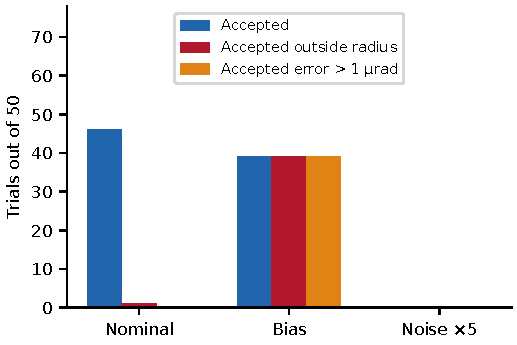
\includegraphics[width=\columnwidth]{premise_sensitivity.pdf}
\caption{Separate preserved affine-drift sensitivity, 50 paired seeds per condition. Counts are rebuilt from per-run rows into one table. ``Outside radius'' and ``error above $1\um$'' are different endpoints. This dataset is not the low-noise, nondeclining-gain confirmation.}
\label{fig:sensitivity}
\end{figure}

\begin{table}[t]
\caption{Premise failures and evidence-supported response. Refusal requires available evidence; an unmodeled violation can remain undetected.}
\centering\footnotesize
\begin{tabular}{@{}p{.27\columnwidth}p{.66\columnwidth}@{}}\toprule
Issue & Consequence / observed or analytic scope\\\midrule
Angle bias & Violates zero-bias contract; 39/39 accepted biased fits miss radius in separate sensitivity. Residual may remain small.\\
Heavy tails & Gaussian mission quantile invalid; adverse-time stress fails event calibration. No tail-robust theorem.\\
Between-set actuator & Interface refuses declared nonmember. Grid success does not certify a continuum.\\
Changing offset / faster gain loss & Breaks reference identity/window lower slope. Historical failures are retained as out-of-model.\\
Possible clamp activation & Linear RK4 enclosure unavailable; reject candidate. Simulations with clips do not extend the theorem.\\
Expired / incomplete evidence & Failure-closed metadata refusal; authority must establish truth of references.\\
Late mission start & New wrapper refuses insufficient remaining horizon. Baseline experiments retain 30 incomplete probes per method at reverse midpoint.\\\bottomrule
\end{tabular}
\label{tab:violations}
\end{table}

\subsection{Related architecture comparisons}
At region~1's midpoint, parameter KF selects and accepts all 600 fits, with 15 accepted offsets outside its approximate radius. Mean angular excitation is $74.747\ \mu$rad$^2$~s, versus 8.331 for UAD. The observed acceptance difference favors the filter; the excitation difference favors UAD in these settings. Neither covariance is exact, and the different waveforms and acceptance rules prevent attributing the difference solely to estimator architecture. Both have zero outage here, so no service-performance superiority over the filter is established.

At the reverse midpoint, parameter KF selects 558 probes and completes/accepts 528 fits. The remaining 30 are still probing at the mission end, not rejected fits. ES also selects 558 with 30 incomplete, and its completed trajectories are tracking results without diagnostic fit acceptance. At the first midpoint, ES angular excitation is 42.381, again with zero observed outage. Figure~\ref{fig:matched} compares common measurable endpoints without rewarding tracking as correct diagnosis.

Faithful comparisons with the original published constrained-AFD or safety-filtered-ES systems remain incomplete. The public guaranteed-AFD implementation \cite{massacode} is identified, but its CORA/solver dependencies are unavailable on the active path. The supplied dependency audit and mapping notes make this blocker explicit. The present KF and ES are conventional adapted architectures; they must not be represented as full reproductions of \cite{guo,massa,safees}.

\begin{figure*}[t]
\centering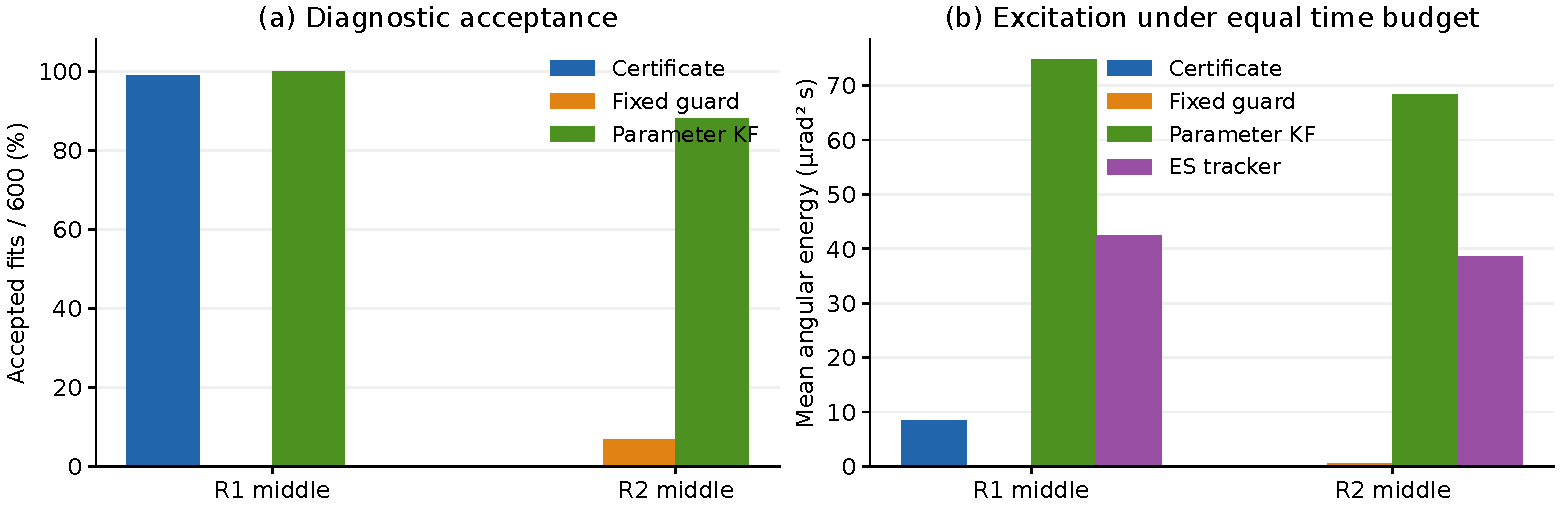
\includegraphics[width=\textwidth]{matched_confirmation.pdf}
\caption{Midpoint comparisons under the same maximum 2.88-s excitation time. Accepted-fit rates and angular excitation are different endpoints. ES is shown only for excitation because it does not produce diagnostic fits. All methods have zero sampled outage in these settings. Full below/above controls and completion counts appear in Table~\ref{tab:matched}.}
\label{fig:matched}
\end{figure*}

\section{Discussion}
The certificate enables a specific engineering decision: under credible contracts, a planner may collect diagnostic data while respecting a declared sampled service budget. At the first midpoint, it supplies evidence where the fixed margin abstains, with much smaller angular excitation than the larger-waveform parameter filter. This is useful diagnostic access on a working link. It does not establish a faster repair, a correct diagnosis for every fit, or an improvement across all possible fault/noise regimes.

The converse admission result explains why conservatism must be evaluated alongside permission. A fixed guard substitutes an unproved radius for the model-derived one. If this fixed value is larger than the model enclosure, it can reject probes the certificate allows; if smaller, it can allow probes the certificate refuses. The reverse-region results show that these extra heuristic admissions need not fail in the tested trajectories. A proof is about all allowed uncertainty realizations under its hypotheses, while successful simulation samples a restricted subset. Neither statement cancels the other.

The large median slack, about $.658p_{\min}$, is a design cost. Initial angular uncertainty can dominate even when actual offset is zero. A lower divergence bound magnifies worst-case power loss. The mission-wide sensor event grows more restrictive as horizon or channel count increases, and the maximum over finite actuators adds motion uncertainty. The nondeclining-gain requirement in the selected favorable region removes another major loss term. A hardware identification program might shrink these contracts, but substituting tighter assumptions without evidence would create apparent performance rather than a justified improvement.

The estimator has a different operating envelope. Twenty-six accepted-radius misses at the first midpoint remain visible despite high acceptance and zero outage. A future method could separate estimator and permission design more rigorously, for example through validated errors-in-variables inference or independently calibrated confidence sets. Such work has not been completed here, and the present paper does not relabel approximate GLS as exact inference. Bias cannot be fixed by more excitation alone when its optical effect is structurally indistinguishable from offset.

Some broader recovery outcomes are unfavorable to UAD. In the distinct preserved nominal affine-drift comparison, its mean outage is 5.0324~s with 46/50 acceptances, versus 4.2420~s and 50/50 for the earlier DAP selector. Time-matched ES has 9.8404~s outage there, whereas native eight-second ES has 4.2676~s and much larger excitation. These results, retained in the supplement, answer a different question than admission on an already functioning link. They prevent the selected frontier findings from being promoted to global recovery superiority.

The supervisory contract makes these boundaries operationally explicit. Missing evidence should result in refusal; a model/measurement breach should invalidate the permission and request a separately validated fallback. However, neither reference strings nor shadow monitoring establish that physical assumptions are true. A receiver/actuator calibration and fault-window evidence process is therefore part of the intended deployment architecture, not a property silently supplied by the mathematical certificate.

\section{Limitations and Scope}
The plant, optics and sensing remain assumed rather than calibrated against a receiver and actuator. No hardware-in-the-loop, flight or industrial deployment is demonstrated. The six-model uncertainty set excludes continuous inertia/lag intervals; intermediate simulations do not enlarge the certified set. Source dynamics are a held-input RK4 sampled model with unrounded arithmetic bounds, and the theorem does not cover intersample threshold crossings.

The sensor event requires correct marginal tails, scales and zero bias for the full declared horizon. It cannot be reused indefinitely across multiple missions without appropriate risk accounting. Fixed offset and divergence and the specified gain-decline bound must remain valid throughout the probe. A supervisor cannot infer all these hypotheses from the same noisy data it is using to diagnose an unknown fault. Unobserved violations can escape monitoring.

The evaluation is development-guided and deliberately concentrated on admission boundaries. The baseline extension is frozen after the original outcomes, equal time does not equal equal excitation, and its adapted implementations do not constitute faithful reproductions of all close published methods. Full-text access and system-level mapping remain necessary for the closest recent optical work. No independent external mathematical review or exhaustive novelty search has been completed. These limitations preclude a claim of established Transactions novelty, physical safety, flight readiness or universal superiority.

Source attribution and content-assistance records are supplied. The repository's API reports no license; attribution alone does not establish redistribution rights. Human source-rights confirmation and approval of the author list, original contribution, disclosure and final content remain submission prerequisites. No author names, institutional affiliations or approvals are invented.

\section{Conclusion}
A reference-relative optical bound, simultaneous sensor event and finite-model actuator enclosure provide a conditional sampled probe-authorization rule. The study demonstrates additional diagnostic access in one restricted region, conservative refusal in the converse region, and substantial excitation/acceptance tradeoffs against adapted parameter filtering and tracking baselines. Zero observed outage does not validate a heuristic guard or a physical failure target. Approximate estimator confidence, hardware calibration, continuous actuator uncertainty and post-probe recovery remain separate unresolved problems.

\section*{Reproducibility}
The supplementary material supplies complete protocols, per-run rows, all new raw traces, independent calculation reports, symbolic identities, unit checks, stage-enclosure details, tests and source hashes. Earlier datasets and statistical corrections are preserved and identified separately; their records are not silently pooled with the 14,400 matched runs. The implementation and complete reproducibility package are identified by the supplied release manifest rather than an invented accepted-paper status.

\section*{Acknowledgments and AI-Use Disclosure}
OpenAI Codex assisted the mathematical formulation and checking, algorithm implementation, experimental scripts, analysis, literature screening, figures and drafting of Sections I--X and the supplementary material. MATLAB generated the recorded plant simulations; separate Python calculations supplied numerical replay and exact-algebra checks. This assistance is substantive and is disclosed under IEEE guidance \cite{aipolicy}. No independent human review is implied. Human authors must verify and take responsibility for the final scientific content, attribution and permissions before submission.

\begin{thebibliography}{99}
\bibitem{guelman} M. Guelman \emph{et al.}, ``Acquisition and pointing control for inter-satellite laser communications,'' \emph{IEEE Transactions on Aerospace and Electronic Systems}, vol. 40, no. 4, pp. 1239--1248, 2004, doi: \href{https://doi.org/10.1109/TAES.2004.1386877}{\nolinkurl{10.1109/TAES.2004.1386877}}.
\bibitem{guo} Y. Guo, Q. Liu, Z. Wang, Z. Zhang \emph{et al.}, ``Active fault diagnosis for linear stochastic systems subject to chance constraints,'' \emph{Automatica}, vol. 156, Art. no. 111194, 2023, doi: \href{https://doi.org/10.1016/j.automatica.2023.111194}{\nolinkurl{10.1016/j.automatica.2023.111194}}.
\bibitem{massa} N. Massa, J. A. Paulson, ``Optimal input design for guaranteed fault diagnosis of nonlinear systems: An active deep learning approach,'' \emph{Control Engineering Practice}, vol. 153, Art. no. 106118, 2024, doi: \href{https://doi.org/10.1016/j.conengprac.2024.106118}{\nolinkurl{10.1016/j.conengprac.2024.106118}}.
\bibitem{safees} A. Williams, M. Krstic, A. Scheinker, ``Semiglobal Safety-Filtered Extremum Seeking With Unknown CBFs,'' \emph{IEEE Transactions on Automatic Control}, vol. 70, no. 3, pp. 1698--1713, 2025, doi: \href{https://doi.org/10.1109/TAC.2024.3469785}{\nolinkurl{10.1109/TAC.2024.3469785}}.
\bibitem{yan} K. Yan, B. Guo, Y. Zhou, X. Xue \emph{et al.}, ``Link-Margin-Aware joint parameter optimization for scanning and acquisition of optical inter-satellite link,'' \emph{Optics Communications}, vol. 616, Art. no. 133342, 2026, doi: \href{https://doi.org/10.1016/j.optcom.2026.133342}{\nolinkurl{10.1016/j.optcom.2026.133342}}.
\bibitem{actuators} M. Milaševičius, L. Mačiulis, ``A Review of Mechanical Fine-Pointing Actuators for Free-Space Optical Communication,'' \emph{Aerospace}, vol. 11, no. 1, Art. no. 5, 2024, doi: \href{https://doi.org/10.3390/aerospace11010005}{\nolinkurl{10.3390/aerospace11010005}}.
\bibitem{baeck} K. Baeck, J. Wi, H. Yoon, ``Analytic pointing error evaluation on nano-satellite laser communication system,'' \emph{Optics Communications}, vol. 559, Art. no. 130419, 2024, doi: \href{https://doi.org/10.1016/j.optcom.2024.130419}{\nolinkurl{10.1016/j.optcom.2024.130419}}.
\bibitem{nasa} NASA Small Spacecraft Systems Virtual Institute, ``State-of-the-art small spacecraft technology: Communications.'' \href{https://www.nasa.gov/smallsat-institute/sst-soa/soa-communications/}{NASA communications overview}; accessed Oct. 23, 2026.
\bibitem{oh} D. Oh, J.-H. Noh, ``Uncertainty Cone Design for Spiral-Scan Optical Acquisition With Time-Correlated Retries,'' \emph{IEEE Transactions on Aerospace and Electronic Systems}, vol. 62, pp. 17450--17464, 2026, doi: \href{https://doi.org/10.1109/TAES.2026.3733932}{\nolinkurl{10.1109/TAES.2026.3733932}}. Publisher abstract/metadata assessed; full-text reproduction unavailable.
\bibitem{es} M. Krstić, H. Wang, ``Stability of extremum seeking feedback for general nonlinear dynamic systems,'' \emph{Automatica}, vol. 36, no. 4, pp. 595--601, 2000, doi: \href{https://doi.org/10.1016/S0005-1098(99)00183-1}{\nolinkurl{10.1016/S0005-1098(99)00183-1}}.
\bibitem{source} Satellite-Optical-Fault-Recovery, source terminal model and V2 implementation, local archived snapshot \texttt{0bc453ffa0ad}. \href{https://github.com/kaushalrog/Satellite-Optical-Fault-Recovery}{Source repository}; accessed Oct. 23, 2026.
\bibitem{massacode} Paulson Laboratory, ``Guaranteed\_AFD\_ADL: Author implementation,'' accessed Oct. 23, 2026. [Online]. Available: \url{https://github.com/PaulsonLab/Guaranteed_AFD_ADL}
\bibitem{aipolicy} IEEE Author Center, ``Submission and peer review policies: Use of AI by authors.'' \href{https://journals.ieeeauthorcenter.ieee.org/become-an-ieee-journal-author/publishing-ethics/guidelines-and-policies/submission-and-peer-review-policies/}{IEEE policy}; accessed Oct. 23, 2026.
\end{thebibliography}

\end{document}
